
\subsection{Part-of-speech tagging}

This section will go into the details of the Part-of-speech task, what the
specifics are, considerations in regards to the data used, any issues we came
across, and the results of our experiments.

\subsubsection{Task definition}

The Part-of-Speech task is a classification task where the objective is to label
each word in a sentence with it's corresponding part-of-speech label such as
noun, verb, adjective, etc. For example, the sentence ``Our work is done'' would be
labeled ``determiner noun auxiliary verb''.

For our dataset, there are around 17 different labels, but some languages don't
use all of them. The same words can have different labels in different context,
so the classifier should be able to figure out which label is a better fit on a
sentence by sentence basis. Simply remembering that word $X$ has label $Y$
wouldn't be able to generalize very well.

The performance of a classifier for the POS task is the simple accuracy of the
predictions. Since there is no label that is a lot more common than others,
guessing randomly would result in a score approximate to $\sim\frac{1}{17}$.

The POS task is relevant to solve since we want machines to be able to
understand the same nuances in natural language as we can. While a lot of people
would have a hard time performing better on the task than a machine would,
everybody understand the difference between how the word ``bear'', functions in
the sentence ``She saw a bear'' and ``Your efforts will bear fruits''
(\cite{medium-pos-intro}). Achieving better results on this task results in
machines better being able to understand natural language.

The state of the art model for POS based off of (\cite{aclweb-pos-state}) is
(\cite{akbik2018coling}) which is a Bi-LSTM-CRF model similar to what we have
made. Based on the defaults we can see from their source code that they use an
embedding size of 100, a single layer Bi-LSTM, mini-batch of 32, patience of 3,
SGD with a learning rate of 0.1, and dropout 0.5, however the specifics hidden
size is unclear. Many of their hyperparameters are the same as what we use, but
they could use other values for their state of the art model. 

Where their model definetely stands out is their use of what they call
``contextual string embeddings'', which are character embeddings, but they use
characters from not just the target word, but words before and after it in the
sentence. Every character from the beginning of the sentence, to the end of the
word is given to a forward language model. And every character from the end of
the sentence, to the beginning of the word is given to a backwards language
model. These language models are pre-trained, and the result of each model is
concatenated to form the complete embedding. 

Their model is evaluated on the Wall Streets Journal datasets achieves a 97.85\%
accuracy, 0.21\% percent points above the previous best model by
(\cite{choi2016dynamic}). Meaning the new model would make $\sim8.9\%$ fewer
errors on the test set.

\subsubsection{Data}\label{sec:experiments-pos-data}

For this task we used datasets from (\cite{universaldependencies}) which has a
broad selection of languages with multiple datasets (called treebanks) in each.
The datasets are all in the CoNNL-U format, but are created from different types
of sources. The source types are given as tags such as news, legal, blog, wiki,
etc. As it is unclear how much of the data is made from each of the sources
given, we prefered datasets made from single source types to keep the datasets
similar to the best of our abilities.

Since the datasets are already split, these were concatenated before splitting
into our own sizes. Concatenation happened using the command \code{cat *.conllu >
combined.conllu}, since the convention for the datasets is to name the files
something with train, test, and dev, the assumed order of the files is dev,
test, and train. Meaning that if the dev set (eg.\ the validation set) contains
5000 sentence, only these were used in our datasets, and none of the sentences
from the test or training sets would be used. No guarantees however were made to
guarantee this ordering, so depending on the naming conventions used in the
specific treebanks this may differ. This shouldn't matter however since there
shouldn't be any difference between the data in the different files.

Some datasets, such as the Norwegian dataset, contains contractions alongside
the individual words. Since the contration is usually unlabelled in the datasets
these were simply removed from the data for ease of parsing. This has the
obvious consequence that the models are not trained on the contractions of words
which are often more commonly used. This however shouldn't affect the
comparisons between word orderings since contractions shouldn't affect these and
the test data would also be using the same convention where contractions are
split. An alternative approach would be to create two sentences, one using the
contraction and another without. This would be a way to extend the dataset and
learn to properly tag both the individual words and their contraction.

The treebanks we selected were all made from news, where some used additional
sources such as non-fiction and spoken. A list of the languages, their
respective treebank selected, and their tags is given below.

* Arabic,   PADT, news

* Hindi,    HDTB, news

* Urdu,     UDTB, news

* Japanese, GSD, blog, news

* Danish,   DDT, fiction, news, non-fiction, spoken

* Norwegian,Bokmaal, blog, news, non-fiction

* Russian,  SynTagRus, fiction, news, non-fiction

The distribution of tokens, labels, etc.\ is given in Figure~\ref{}.

\subsubsection{Model convergence}

Looking at the results of the experiments, we mainly focus on the case where the
models were trained with early stopping. As such, we where
interested in seeing how the models converged with different batch sizes aswell
as with and without the CRF layer. The average number of epochs run for each
framework implementation is shown in Table~\ref{table:epochs-run-pos}.

\begin{table}[h!]
    \centering
    \begin{tabular}{l c c c|c c c}
        \toprule
        \multirow{2}{*}{\bfseries Batch size}     &
        \multicolumn{3}{c}{\bfseries Bi-LSTM}     &
        \multicolumn{3}{c}{\bfseries Bi-LSTM-CRF} \\
        \cmidrule(lr){2-7}
        & DyNet & PyTorch & TensorFlow
        & DyNet & PyTorch & TensorFlow \\
        \cmidrule(lr){1-7}
         1 & 13.60 & 21.44 & 36.43 & 13.26 &  8.09 &  5.23 \\
         8 & 17.31 & 39.86 & 49.71 & 16.55 & 16.20 &  7.91 \\
        32 & 22.57 & 48.83 & 50.00 & 23.78 & 22.40 & 10.66 \\
        \bottomrule
    \end{tabular}
    \caption{Average of epochs run across all seeds and languages when trained
        with early stopping.
    }\label{table:epochs-run-pos}
\end{table}

From the data it is clear, that an increase in batch size also means that the
model takes longer to converge. This is expected, as the number of
backpropagation operations decrease when the input data is split into larger
mini-batches (eg.\ when working with 4000 sentences and a batch size of 1, each
epoch will update its weights 4000 times. This number drops to
$\frac{4000}{32}=125$ when the batch size is 32).

We also see, that adding a CRF layer dramatically decrease the time it takes for
the models to converge. With the standard \texttt{Bi-LSTM} model implemented in
TensorFlow, none of our experiments reached a point of convergence within the
upper bound on the number epochs, and for PyTorch with batch size 32 and
TensorFlow with batch size 8 the average number also indicate that only very few
training sessions reached the point of convergence before the epoch limit. This
also suggests, that we set the upper bound to strict.

It is a completely different story for the \texttt{Bi-LSTM-CRF} models. Here,
all experiments terminated early and the relation between the frameworks
changed.  DyNet had an almost identical epoch average, but PyTorch saw a more
than 50\% drop and for TensorFlow the drop was more than 80\%. The explanation
for this could be, that the 2 layer \texttt{Bi-LSTM} of the DyNet implementation
is a more efficient model than the regular \texttt{Bi-LSTM} with only 1 layer,
and that the addition of a CRF layer is insignificant (in terms of the time it
takes to find a convergence point). For the PyTorch and TensorFlow
implementation, however, it seems that the CRF layer greatly helps the
sequential model to converge.

We do find it odd, though, that the TensorFlow implementation on average across
batch sizes takes less than 10 epochs to find a satisfying convergence point.

\subsubsection{Accuracy}

When we turn our attention to the accuracy achieved by the models, we see the
results reflect the epoch numbers. In
Figure~\ref{chart:acc-by-batch-and-lang-pos} the results are plotted
according to batch size and language. A table of all the data can be found in
Table~\ref{table:acc-total-pos}.

\begin{figure}[h!]
    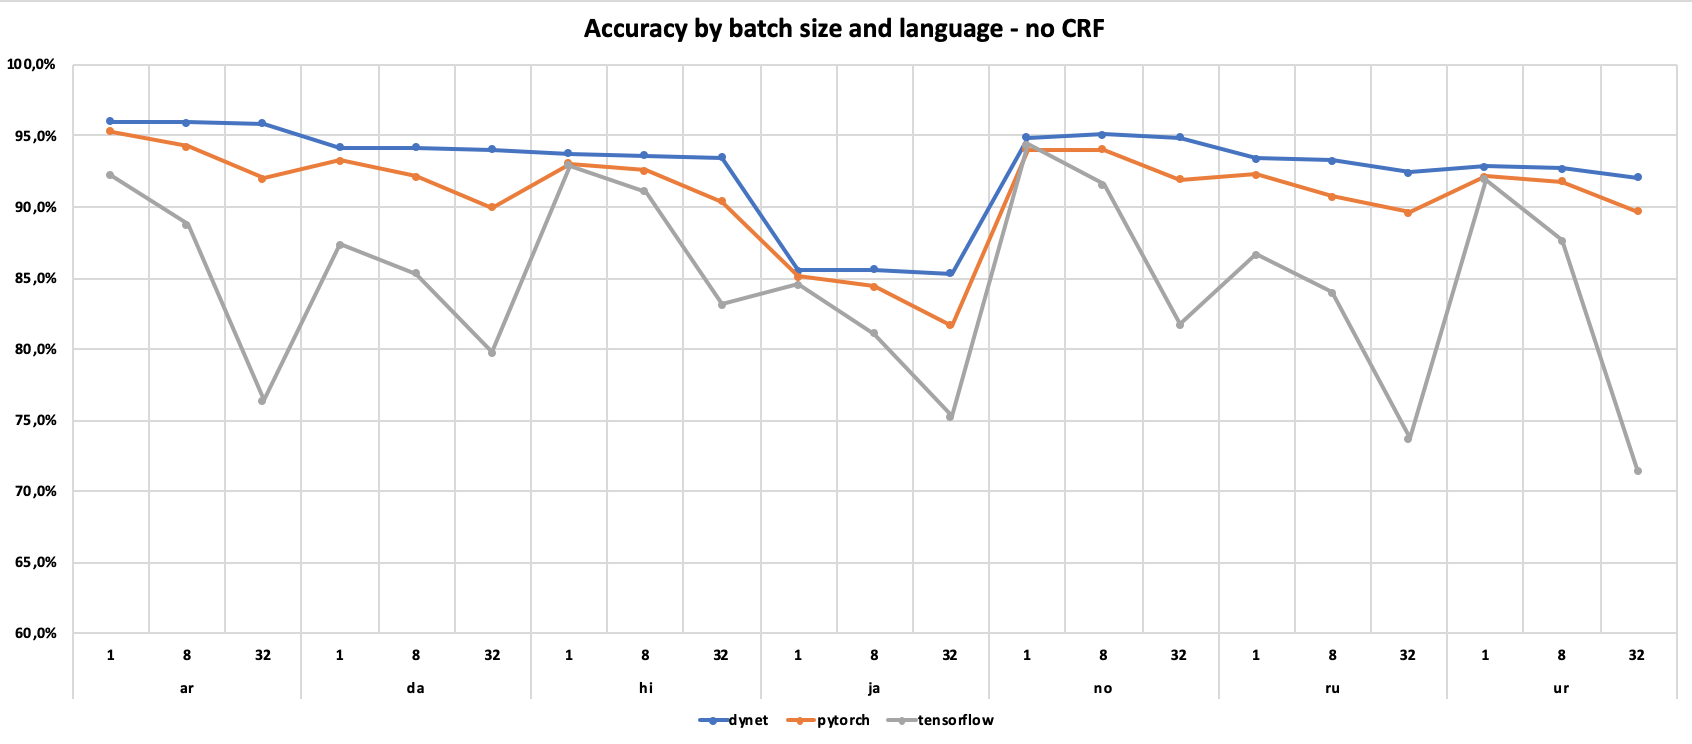
\includegraphics[width=\textwidth]{accuracy-pos-no-crf}
    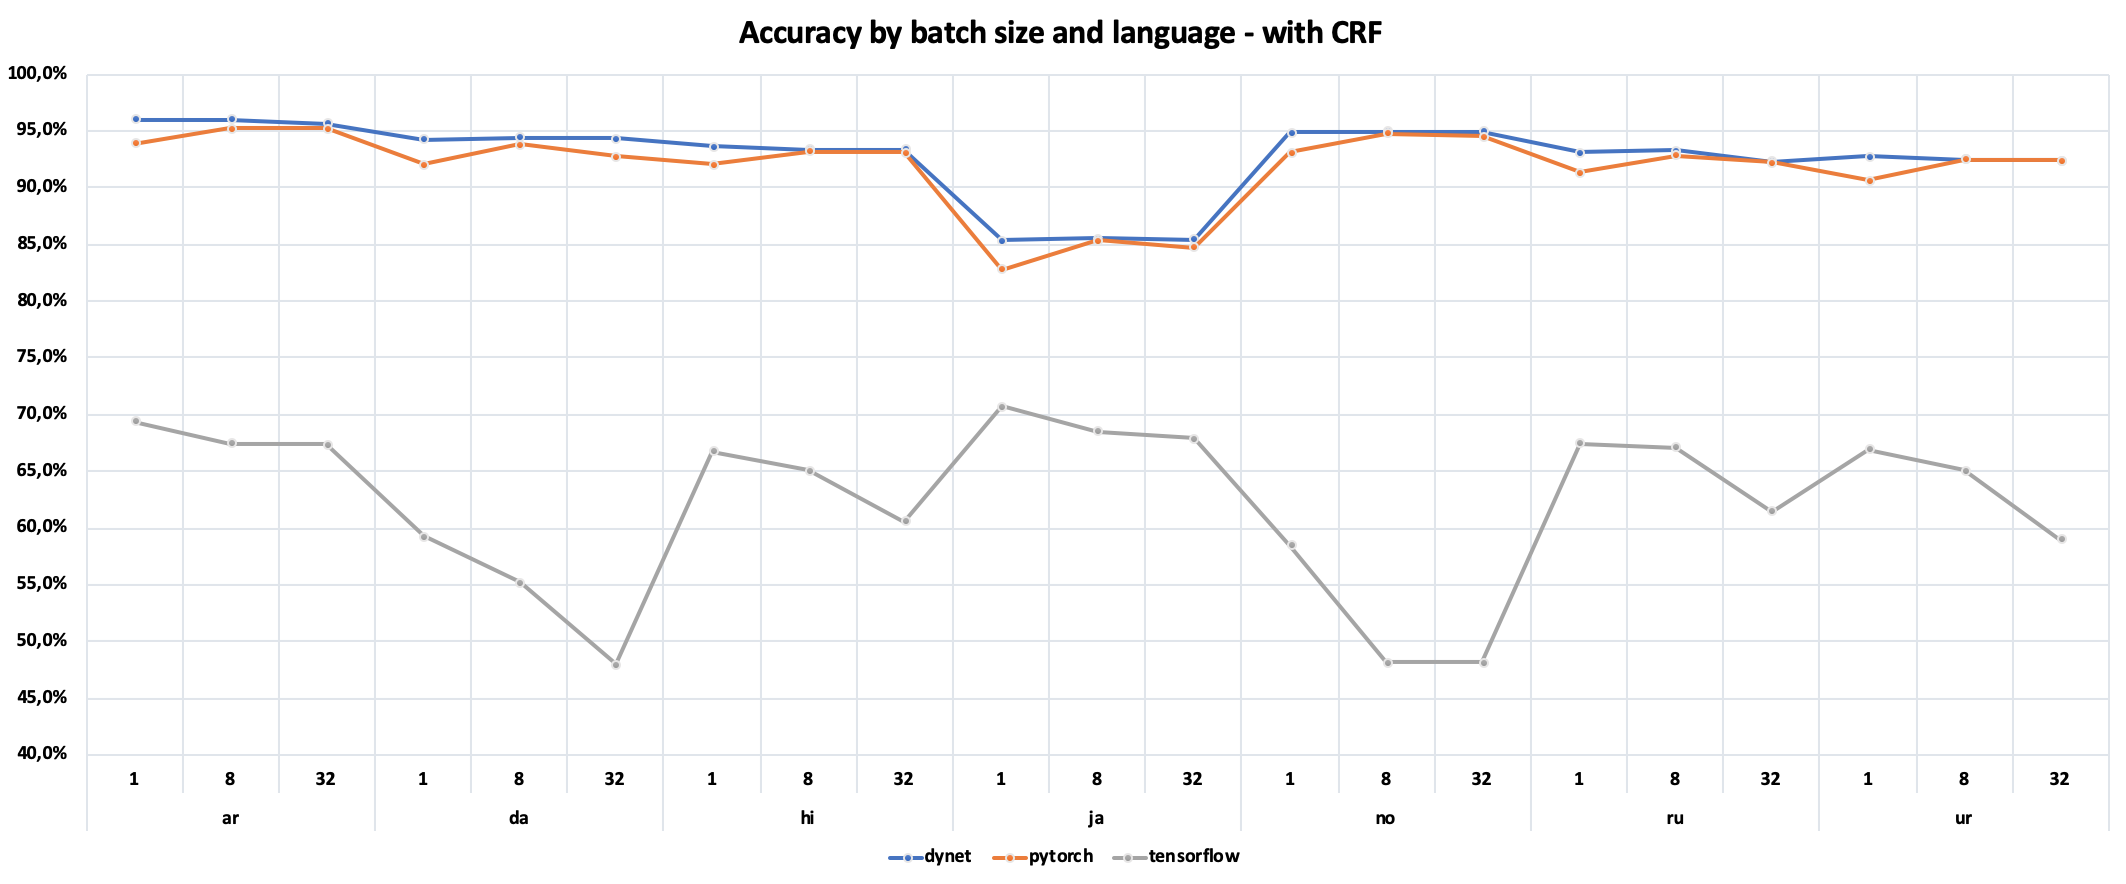
\includegraphics[width=\textwidth]{accuracy-pos-with-crf}
    \caption{Average accuracy across seeds with early stopping and a maximum of
        50 epochs. The x-axis is batch size 1, 8 and 32 for all languages in the
        experiments. Top: Results for \texttt{Bi-LSTM}. Bottom: Results for
    \texttt{Bi-LSTM-CRF}. \textbf{NB:} Notice different y-axises.
    }\label{chart:acc-by-batch-and-lang-pos}
\end{figure}

\begin{table}[h]
    \centering
    \begin{tabular}{c l c c c|c c c}
        \toprule
        \multirow{2}{*}{\bfseries Language} &
        \multirow{2}{*}{\bfseries Batch size} &
        \multicolumn{3}{c}{\bfseries Bi-LSTM} &
        \multicolumn{3}{c}{\bfseries Bi-LSTM-CRF} \\
        \cmidrule(lr){3-8}
        && DyNet & PyTorch & Tensorflow & DyNet & PyTorch & Tensorflow \\

        \cmidrule(lr){1-8}
        \multirow{3}{*}{\bfseries ar}
        &  1 & \underline{\textbf{96.0\%}} & \underline{95.3\%} & \underline{92.2\%} & \underline{\textbf{96.0\%}} & 93.9\% & 69.4\% \\
        &  8 & \underline{\textbf{96.0\%}} & 94.3\% & \underline{88.8\%} & \underline{\textbf{96.0\%}} & \underline{95.2\%} & 67.5\% \\
        & 32 & \underline{\textbf{95.8\%}} & 92.0\% & \underline{76.4\%} & \underline{\textbf{95.8\%}} & \underline{95.3\%} & 67.4\% \\

        \cmidrule(lr){1-8}
        \multirow{3}{*}{\bfseries da}
        &  1 & 94.2\% & \underline{93.2\%} & \underline{87.4\%} & \underline{\textbf{94.3\%}} & 92.1\% & 59.3\% \\
        &  8 & 94.2\% & 92.2\% & \underline{85.4\%} & \underline{\textbf{94.4\%}} & \underline{93.8\%} & 55.2\% \\
        & 32 & 94.1\% & 90.0\% & \underline{79.8\%} & \underline{\textbf{94.3\%}} & \underline{92.8\%} & 47.9\% \\

        \cmidrule(lr){1-8}
        \multirow{3}{*}{\bfseries hi}
        &  1 & \underline{\textbf{93.8\%}} & \underline{93.0\%} & \underline{92.9\%} & 93.6\% & 92.0\% & 66.8\% \\
        &  8 & \underline{\textbf{93.7\%}} & 92.6\% & \underline{91.1\%} & 93.4\% & \underline{93.2\%} & 65.0\% \\
        & 32 & \underline{\textbf{93.5\%}} & 90.4\% & \underline{83.1\%} & 93.4\% & \underline{93.1\%} & 60.6\% \\

        \cmidrule(lr){1-8}
        \multirow{3}{*}{\bfseries ja}
        &  1 & \underline{\textbf{85.5\%}} & \underline{85.1\%} & \underline{84.6\%} & 85.4\% & 82.8\% & 70.8\% \\
        &  8 & \underline{\textbf{85.6\%}} & 84.4\% & \underline{81.1\%} & 85.5\% & \underline{85.3\%} & 68.5\% \\
        & 32 & \underline{\textbf{85.3\%}} & 81.7\% & \underline{75.3\%} & \underline{\textbf{85.3\%}} & \underline{84.7\%} & 67.9\% \\

        \cmidrule(lr){1-8}
        \multirow{3}{*}{\bfseries no}
        &  1 & \underline{\textbf{94.9\%}} & \underline{94.0\%} & \underline{94.4\%} & \underline{\textbf{94.9\%}} & 93.1\% & 58.5\% \\
        &  8 & \underline{\textbf{95.1\%}} & 94.0\% & \underline{91.6\%} & 95.0\% & \underline{94.8\%} & 48.1\% \\
        & 32 & \underline{\textbf{94.9\%}} & 91.9\% & \underline{81.8\%} & \underline{\textbf{94.9\%}} & \underline{94.5\%} & 48.1\% \\

        \cmidrule(lr){1-8}
        \multirow{3}{*}{\bfseries ru}
        &  1 & \underline{\textbf{93.4\%}} & \underline{92.3\%} & \underline{86.7\%} & 93.1\% & 91.3\% & 67.5\% \\
        &  8 & \underline{\textbf{93.3\%}} & 90.7\% & \underline{84.0\%} & \underline{\textbf{93.3\%}} & \underline{92.8\%} & 67.1\% \\
        & 32 & \underline{\textbf{92.4\%}} & 89.6\% & \underline{73.7\%} & 92.3\% & \underline{92.3\%} & 61.5\% \\

        \cmidrule(lr){1-8}
        \multirow{3}{*}{\bfseries ur}
        &  1 & \underline{\textbf{92.9\%}} & \underline{92.1\%} & \underline{91.9\%} & 92.7\% & 90.6\% & 67.0\% \\
        &  8 & \underline{\textbf{92.7\%}} & 91.8\% & \underline{87.6\%} & 92.5\% & \underline{92.5\%} & 65.0\% \\
        & 32 & 92.1\% & 89.7\% & \underline{71.4\%} & \underline{92.2\%} & \underline{\textbf{92.4\%}} & 59.0\% \\
        \bottomrule
    \end{tabular}
    \caption{%
      Accuracy results on POS data by language and batch size.
      Bold: highest accuracy for batch size plus language.
      Underline: highest accuracy for framework between
      \texttt{Bi-LSTM} and \texttt{Bi-LSTM-CRF}.
    }\label{table:acc-total-pos}
\end{table}


There is a clear outlier in the data and that is the TensorFlow implementation.
Especially for the \texttt{Bi-LSTM-CRF} model, the this yields significantly
lower results and a pattern that does not resemble that of the other two. A good
example is the fact that for Japanese, both the DyNet and the PyTorch
implementation perform worse than they do for any other language, whereas the
TensorFlow one has its best accuracy on Japanese with a batch size of 1 and  a
consitently above-average score for batch size 8 and 32, though all 3 results
are more than 10\% lower than those of DyNet and PyTorch.

Taking into account the unusually low number of epochs it trained before
seemingly converging, these irregularities in our TensorFlow
\texttt{Bi-LSTM-CRF} combined with how similar the DyNet and PyTorch
implementations behave, leads us to suspect that there is an error in our CRF
implementation in TensorFlow. Section~\ref{sec:discuss_models} elaborates on this.

For the rest of the results, there seem to be a correlation beween accuracy and
number of epochs trained.

For example, the results show that the non-CRF models perform quite simiar for
most languages when the batch size is 1 (except for the TensorFlow
implementation, which underperforms severely for arabic, danish and russian).
This is in compliance with the finding that for a batch size of 1, all models
terminated training before reaching the maximum number of epochs. The
similarities in performance is a good measurement that these models found a
somewhat optimal tuning of their respective weights.

In the cases where the models did not get to properly converge (ie.\ the
implementation of \texttt{Bi-LSTM} in TensorFlow with batch size 8 and 32 and in
PyTorch with batch size 32), the accuracies achieved are not as good as those of
the DyNet implementation, which terminated training before 25 epochs for
all batch sizes. Its also worth noticing, that the PyTorch implementation with
batch size 8 is also doing notably worse than the corresponding DyNet one, even
though it did seem to converge, albeit at a higher epoch number of 39.86. Since
TensorFlow with a batch size of 1 is also doing worse on average and spent more
than 30 epochs converging, we may see that the eventual convergence after 30
epochs is in higher risk of ending up in a sub-optimal state (ie.\ gets stuck in
a local minima that is not optimal).

For the \texttt{Bi-LSTM-CRF} models, the DyNet and the PyTorch implementation
performs nearly identical, with a small advantage for DyNet in most cases. It is
however interesting to see, that PyTorch gets a significant improvement from the
CRF layer and outperforms its \texttt{Bi-LSTM} model for all batch sizes of 8
and 32. On the other hand, a batch size of 1 performs worse in all cases with
the CRF layer. This could mean that in training a CRF model, backpropagation
hurts from updating on too small a sample size at a time. A larger batch size
should generally make the model less dependent on singular cases and thus better
generalizing the tuning of its weights (\cite{falcon2018lstms}).

The same pattern is not seen for the DyNet implementation, however. Here, the
\texttt{Bi-LSTM-CRF} actually performs marginally worse than the regular
\texttt{Bi-LSTM}. But this does not change the fact, that for all but one
experiment, the DyNet implementation achieves the highest accuracy of all (the
exception being Urdu at batch size 32 where \texttt{Bi-LSTM-CRF} in PyTorch
beats it by 0.02\%). We believe this is an indication, that a 2 layer
bidirectional LSTM model performs comparably to single layer bidirectional LSTM
model with CRF, and that adding a CRF layer to a 2 layer bidirectional LSTM
model has negligible effect but increases training time.

\pagebreak
